\documentclass[12pt]{article}
\usepackage{geometry}
\usepackage{graphicx}
\usepackage{amssymb}
\usepackage{ bm }
\usepackage{amsmath}
\usepackage{hyperref}
\usepackage{caption}
\usepackage{algorithm}
\usepackage[noend]{algorithmic}
%\usepackage[noend]{algcompatible}

\usepackage{tikz}
\usetikzlibrary{shapes,arrows,shadows}
%\usepackage{amsmath,bm,times}
\newcommand{\mx}[1]{\mathbf{\bm{#1}}} % Matrix command
\newcommand{\vc}[1]{\mathbf{\bm{#1}}} % Vector command

\hypersetup{ 
    colorlinks=true,
    linkcolor=blue,
    filecolor=magenta,      
    urlcolor=blue,
    citecolor=blue
}


%\usepackage[linesnumbered,ruled]{algorithm2e}


\title{Deep Q-Learning for Event Summarization }

\author{
	Francisco Javier Arceo \\ \href{mailto: fja2114@columbia.edu}{\small fja2114@columbia.edu} 
		\and  
	Chris Kedzie \\ \href{mailto: kedzie@cs.columbia.edu}{\small kedzie@cs.columbia.edu} 
	}

\begin{document}
\maketitle

\begin{abstract}
We present a streaming extraction policy for multi-document summarization learned using a deep reinforcement learning recurrent neural network architecture. The rewards of our network are evaluated through manually reviewed summaries, which allow us to specify an end-to-end framework to optimize our extraction policy.  By using raw text from our articles and mapping words into a higher embedding dimension through our recurrent neural network, we are able to learn a more robust representation than traditional n-gram models. We benchmark our model against random actions, a bag-of-words model, and a bag-of-bigrams model.\footnote{ \url{https://github.com/franciscojavierarceo/DQN-Event-Summarization} }
\end{abstract}

\bibliographystyle{plain}

\section{Introduction}

Recent research in text retrieval  has focused on extractive algorithms to identify important sentences from a large set of documents (e.g., \cite{diazquery}, \cite{kedzie2015predicting}, \cite{garbacea2015university}, and \cite{kedzieextractive}). The approach by \cite{kedzie2015predicting}  has shown that it is possible to select relevant sentences from a massive number of documents on the web to create summaries with meaningful content by adapting classifiers to maximize search policies. These systems operate in a streaming fashion and are capable of evaluating each sentence within each article to decide whether or not to include or ignore the sentence. 

Unfortunately, many of these systems have still been shown to fall short of algorithms that employ simple heuristics \cite{garbacea2015university}, which may be due to inadequate capturing of the rich structure and often idiosyncratic information by traditional n-gram language models.  

In recent years, recurrent neural networks have been used to map textual language to a higher order dimension to represent more powerful features for a variety of different language modeling tasks \cite{mikolov2010recurrent}. These vector representations, also known as embeddings, have proven incredibly powerful on a variety of different natural language processing tasks (e.g., \cite{bengio2003neural}, \cite{sundermeyer2012lstm}, \cite{kim2016character}). For query based retrievals, \cite{diazquery} has shown success in using these embeddings for \emph{ad hoc} information retrieval.

In this paper we show that a deep recurrent neural network with a long short term memory (LSTM) \cite{hochreiter1997long} is able to successfully learn an extractive summary policy by encoding the action, state, and reward into a Q-Learning model, similar to that of  \cite{hausknecht2015deep}. We show the performance of our model on a variety of different metrics and benchmark them against random actions, a bag-of-words multilayered perceptron, and bag-of-bigrams multilayered perceptron.

% Section 3
\section{Extractive Streaming Summarization}

In the extractive streaming summarization task, we are given as input a query (i.e., a short text description of a topic or an event), a document stream, and a time ordered set of sentences relevant to the query. Starting with an initially empty summary,  an extractive, streaming summarization algorithm is intended to examine each sentence in order and, when new and important (relative to the query) information is identified, add that sentence to the summary. 

Implicit to this problem is the notion of system time -- the summarization algorithm can only examine sentences that occur in the stream before the current system time. Advancing the system time gives the algorithm access to more sentences, although in practice the stream is sufficiently large enough that choices have to be made about how much history can be kept in memory. For many domains, e.g., crisis informatics, it is preferable for a summarization algorithm to identify important information as early as possible, and so the objective function should penalize a large disparity between the time a piece of information is first available to the algorithm and the system time at which that information is actually added to the summary.

Previous work in this area has either incremented the system time in fixed increments (e.g., an hour)  \cite{mccreadie2014incremental, kedzie2015predicting} or operated in a fully online setting \cite{guo2013updating,kedzie2016real}. In both cases explicitly modeling the current state of the summary, the stream, and their relationship with the query is quite complicated and exhibits non-linear dynamics that are difficult to characterize in traditional models with manually crafted features.

Additionally, the structured nature of the sentence selection task (sentence selection is highly dependent on the current summary state) suggests that imitation or reinforcement learning are necessary to obtain parity between training and testing feature distributions. 

Early successes of deep reinforcement learning have used convolutional neural networks for video games (e.g., \cite{MnihBMGLHSK16} and \cite{MnihKSGAWR13}) but recent work has leveraged recurrent neural networks for both video-based and text-based gaming environments (e.g., \cite{hausknecht2015deep} and \cite{narasimhan2015language}). 

This leads us to explore Deep Q-Networks (DQN) for three reasons: (1) both the representation and interaction between the stream, summary, and 
query can be learned; (2) the embeddings can learn a more robust semantic representations than classic n-gram models; and (3) by randomly exploring the state space, the $\epsilon$-greedy strategy used in DQN learns a policy that yields more consistency between train and test distributions.

\section{Background}

In the subsequent sections, we outline the architecture of our DQN and define the parameterization of our Q-function for the multi-document summarization task. Our architecture consists of three components: the (1) input, (2) action, and (3) value representations. By specifying these components into our neural network, we are able to develop an end-to-end extraction policy that fully propagates information both forward and backward.

\subsection{States}  

In our architecture a state $s(x_{t},\tilde{y}_{t}, d)$ is a function of the stream $X_d$, $\forall d \in D$, the state of the current summary $\tilde{y}_t$ at system time $t$, and the query $d$. For brevity we will use $s_t$ where the dependence on $x_{t},\tilde{y}_{t},$ and $d$ is assumed. $s_t$ itself is three recurrent neural networks, one for encoding  the summary, the stream, and the query. 

\subsection{Actions} 
The set of possible actions $a_t$ at each time step is $\mathcal{A} = \{select, skip\}$ where $select$ corresponds to adding the current sentence $x_t$ to the summary and incrementing the current system time, or $skip$ where only $t$ is incremented without changing the current summary. Thus, our current predicted summary at time $t$ is defined as

\begin{equation}
	\tilde{y}_{t + 1} =
	\begin{cases}
		\tilde{y}_{t} \cup \{ x_t \},	& \text{if } a_t = select  \\
		\tilde{y}_{t}, 			& \text{if } a_t = skip.
	\end{cases}
\end{equation}
Since $\tilde{y}_t$ grows linearly with the number of selected sentences, we mitigate potential capacity constraints by using a queue to hold the last $K$ elements of the current predicted summary. 

\subsection{Rewards} 
The reward for a given action is measured by the change in ROUGE-N F1 score of the predicted summary $\tilde{y}_{t}$ measured against a gold standard summary $Y$. When only one gold summary reference is used, ROUGE-N Recall is calculated as 

\begin{equation}
 \textrm{ROUGE-NR}(\tilde{y}, Y) = 
    \frac{\sum_{g \in \textrm{ngrams}(Y,N)} 
    \min \left(\textrm{count}(g, \tilde{y}), \textrm{count}(g, Y)\right)}{
    \sum_{g \in \textrm{ngrams}(Y,N)} 
    \textrm{count}(g, Y)
    }
\end{equation}

where $\textrm{ngrams}(Y, N)$ returns the set of ngrams of order $N$ in the summary $Y$ and $\textrm{count}(g, Y)$ is the count of occurrences of ngram $g$ in $Y.$

Similarly, ROUGE-N Precision is calculated as 

\begin{equation}
\textrm{ROUGE-NP}(\tilde{Y}, Y) = 
    \frac{\sum_{g \in \textrm{ngrams}(Y,N)} 
    \min \left(\textrm{count}(g, \tilde{Y}), \textrm{count}(g, Y)\right)}{
        \sum_{g \in \textrm{ngrams}(\tilde{Y},N)} 
        \textrm{count}(g, \tilde{Y})
    }
\end{equation}

and the $F_1$ is simply the harmonic mean of the two:
\begin{equation}
\textrm{ROUGE-NF1}(\tilde{Y}, Y) = \frac{ 2 \times 
\textrm{ROUGE-NP}(\tilde{Y}, Y) \times \textrm{ROUGE-NR}(\tilde{Y}, Y)
}{ \textrm{ROUGE-NP}(\tilde{Y}, Y) + \textrm{ROUGE-NR}(\tilde{Y}, Y) }
\end{equation}

The reward $r$ at time $t$ is 
\begin{equation}
r_t = \textrm{ROUGE-NF1}(\tilde{y}_{t}, Y) -  \textrm{ROUGE-NF1}(\tilde{y}_{t-1}, Y).
\end{equation}
\subsection{Deep Q-Learning}

We define an architecture similar to that of \cite{narasimhan2015language} and map our three inputs (query, sentence, and current predicted summary) into LSTM embeddings according to $\textbf{Figure 1}$. By formulating our extraction task as a Markov Decision Process (MDP) we can express the state-action tuples as transitions states. 

Our extraction policy then takes as input an action $a_t$ in state $s_t$ at time $t$ and returns the expected reward. We initialize our actions and Q-function at random and by taking the optimal action given our expected reward, we are able to iteratively update our Q-function using the Bellman equation \cite{sutton1998reinforcement} satisfying

\begin{equation}
	\hat{Q}_{t+1}(s,a) = \textrm{E}[ r + \gamma \textrm{max}_{a'} \hat{Q}_t(s', a') | s, a]
\end{equation}
where $\gamma \in \mathbb{R}$ is the discount rate applied to future rewards and the expectation is taken over transitions in state $s$ and action $a$. By iterating over the Q-function, it converges asymptotically to the optimal policy, i.e.,  $\hat{Q}_t \rightarrow Q^{*}$ as $t \rightarrow \infty$. In finite iterations we can use a neural network as our function approximator, where our weights, $\theta$, can be optimized using the following loss function

\begin{equation}
	\mathcal{L}_i(\theta_i) =  \textrm{E}_{\hat{s}, \hat{a}}[ \big (y_i - Q(\hat{s}, \hat{a}; \theta_i) \big )^2]
\end{equation}

where 
\begin{equation}
	y_i = \textrm{E}_{\hat{s}, \hat{a}}[ r_i + \gamma \textrm{max}_{a'} Q(s', a' ; \theta_{i-1}) | s', a' ].
\end{equation}

Differentiation of the loss function yields the update equation,

\begin{equation}
	\nabla_{\theta_i} L_i(\theta_i) = \textrm{E}_{\hat{s}, \hat{a}}[ 2  \big (y_i - Q(\hat{s}, \hat{a}; \theta_i) \big ) \nabla_{\theta_{i}}  Q(\hat{s}, \hat{a}; \theta_i)]
\end{equation}
that learns the parameters using stochastic gradient descent with RMSprop \cite{hinton2012lecture} on sampled batches of stored transitions.

\begin{center}

\pgfdeclarelayer{background}
\pgfdeclarelayer{foreground}
\pgfsetlayers{background,main,foreground}
    % Define the layers to draw the diagram
    \tikzstyle{sensor}=[draw, fill=blue!10, text width=5em,  text centered, minimum height=2.0em,drop shadow]
    \tikzstyle{term}=[draw, fill=gray!10, text width=5em,  text centered, minimum height=2.0em,drop shadow]
    \tikzstyle{wa} = [sensor, fill=gray!10, text width=5em,  minimum height=2em, rounded corners, drop shadow]
    \tikzstyle{wa} = [sensor, fill=gray!10, text width=5em,  minimum height=2em, rounded corners, drop shadow]
    \tikzstyle{wa2} = [sensor, fill=gray!10, text width=6em,  minimum height=12em, drop shadow]
    \tikzstyle{om} = [draw, fill=green!05, text width=5em,  text centered, minimum height=2.0em,drop shadow]

\begin{tikzpicture}[scale=0.75, transform shape]
        \node (wa) [wa2] {Joined \textbf{ReLU Layer}  \\ \scriptsize (3 x Embedding) };
        \path (wa.west)+(-3.0 ,  2.0) node (asr1)[sensor] {$Query$ \textbf{LSTM}};
        \path (wa.west)+(-3.0 ,  0.0) node (asr2)[sensor] {$Sentence_t$  \textbf{LSTM}};
        \path (wa.west)+(-3.0 , -2.0) node (asr3)[sensor] {$Summary_t$  \textbf{LSTM}};
        \path (wa.east)+(3.0,  1) node (vote) [term] {\textbf{ReLU} \\ \scriptsize $\{Select\}$ };
        \path (wa.east)+(3.0, -1) node (vote2) [term] {\textbf{ReLU} \\ \scriptsize $\{Skip\}$ } ;
        \path (wa.east)+(6.5,  0) node (output) [om] {\textbf{Select} \\ \scriptsize E[Rouge]} ;

        \path [draw, ->] (asr1.east) -- node [above] {}     (wa.125);
        \path [draw, ->] (asr2.east) -- node [above] {}     (wa.180);
        \path [draw, ->] (asr3.east) -- node [above] {}     (wa.235);
        \path [draw, ->] (wa.east) -- node [above] {}       (vote.west);
        \path [draw, ->] (wa.east) -- node [above] {}       (vote2.west);
        \path [draw, ->] (vote.east) -- node [above] {}     (output.175);
        \path [draw, ->] (vote2.east) -- node [above] {}   (output.185);

     \begin{pgfonlayer}{background}[transparency group,opacity=.5]
            \path (asr1.north  |- asr1.south)+(-2.0, 1.6) node (a) {};
            \path (asr3.west  |- vote.east)+(+10.0, -3.5) node (b) {};
            \path (asr3.west  |- vote.east)+(+10.0, -2.5) node (c) {};
            \path (asr3.east  |- output.east)+(+13, -4.50) node (d) {};
            \path[fill=white!20,rounded corners, draw=black!100, dashed]         (a) rectangle (d);
        \end{pgfonlayer}

     \begin{pgfonlayer}{background}[transparency group,opacity=.5]
            \path (asr1.north  |- asr1.south)+(-1.7, 1.3) node (a) {};
            \path (asr3.west  |- asr3.east)+(+10.0, -3.5) node (b) {};
            \path (asr3.west  |- asr3.east)+(+10.0, -2.5) node (c) {};
            \path (asr3.west  |- asr3.east)+(+2.9, -1.50) node (d) {};
            \path[fill=white!20,rounded corners, draw=blue!100, dashed]         (a) rectangle (d);
        \end{pgfonlayer}

     \begin{pgfonlayer}{background}[transparency group,opacity=.5]
            \path (asr1.north  |- asr1.south)+(2.7, 1.3) node (a) {};
            \path (asr3.west  |- asr3.east)+(+10.0, -3.5) node (b) {};
            \path (asr3.west  |- asr3.east)+(+10.0, -2.5) node (c) {};
            \path (asr3.west  |- asr3.east)+(+11.5, -1.50) node (d) {};
            \path[fill=white!20,rounded corners, draw=gray!100, dashed]         (a) rectangle (d);
        \end{pgfonlayer}

     \begin{pgfonlayer}{background}[transparency group,opacity=.5]
            \path (asr1.north  |- asr1.south)+(7.4, 1.0) node (a) {};
            \path (asr3.west  |- asr3.east)+(+10.0, -3.5) node (b) {};
            \path (asr3.west  |- asr3.east)+(+10.0, -2.5) node (c) {};
            \path (asr3.west  |- asr3.east)+(+11.3, -0.50) node (d) {};
            \path[fill=red!05,rounded corners, draw=black!100, dashed]         (a) rectangle (d);
        \end{pgfonlayer}

     \begin{pgfonlayer}{background}[transparency group,opacity=.5]
            \path (asr1.north  |- asr1.south)+(10.7, 1.3) node (a) {};
            \path (asr3.west  |- asr3.east)+(+10.0, -3.5) node (b) {};
            \path (asr3.west  |- asr3.east)+(+10.0, -2.5) node (c) {};
            \path (asr3.west  |- asr3.east)+(+15.1, -1.50) node (d) {};
            \path[fill=white!20,rounded corners, draw=green!100, dashed]         (a) rectangle (d);
        \end{pgfonlayer}

        \path (wa.west) + (5.8,    2.25)  node (vote.east) {\scriptsize \textbf{Action} }; 
        \path (wa.west) + (5.8,    1.95)  node (vote.east) {\scriptsize $\{argmax(a_t)$\}}; 
        \path (wa.west) + (-2.90, -3.2)  node (vote.east) {Input}; 
        \path (wa.west) + (3.5,    -3.2)  node (vote.east) {State-Action Representation }; 
        \path (wa.west) + (9.30,  -3.2)  node (vote.east) {Output};
        \path (wa.east) + (0.5, -4.2)  node (vote.east) {\textbf{Figure 1: DQN-LSTM Architecture}};
\end{tikzpicture}
\end{center}

\section{Learning an Extraction Policy}
\subsection{Settings}
Since the state of our current summary at time $t$ depends on the state at time $t - 1$, we have to execute our Q-function in the feedforward stage using a single batch to properly update the predicted summary with optimal expected action. During the backpropagation phase we sample random mini-batches from the stored transitions.  We set our embedding dimension to 100, the future discount rate $\gamma$ to 0.50, and the maximum summary length to 300 tokens.

The weights of the Q-function and the action sequence are initialized at random and we randomly explore the state-space for 200 of the 1000 epochs by employing an $\epsilon$-greedy search strategy that decays linearly to a base exploration rate of 0.01 during our action selection. We describe in full detail the training of our DQN-LSTM in $\textbf{Algorithm 1}$.


\begin{algorithm}
    \bf{Input:} { \rm  \{$\mathcal{D}$: Event queries, $X_d$: Input sentences, $N$: Number of epochs\} } \\
    \underline{$\bf{Output: }$ \rm \{$\hat{Q}$: extraction policy, $\tilde{Y}_d$: event summary for query $d$\} }
\begin{algorithmic}[1]
\STATE \rm Initialize action-value function $\hat{Q}$ with random weights
\STATE \rm Initialize memory and summary: $\Gamma, \tilde{Y} =  \{\emptyset \}^{\mathcal{|D|}}_{d=1},  \{\emptyset \}^{\mathcal{|D|}}_{d=1} $
\FOR{$epoch=1,..,N\ $}
	\FOR{query $d \in \mathcal{D}$}
		\STATE $X_{d}, \tilde{Y}_{d}$ = \{Extract $t=1,...,T_d$ ($sentences_d$, $summary_d$)\}
		\FOR{$x_t, \tilde{y}_t \in X_d, \tilde{Y}_d$ }
			\STATE Set $s_t = s(x_t, \tilde{y}_t, d)$
			\STATE $ \forall a_t \in \mathcal{A}(s_t)$ \textrm{compute} $\hat{Q}(s_t, a_t)$ and select $a^{*}_t =$ argmax$_{a_{t}}\hat{Q}(s_t, a_t)$
			\STATE  \textbf{if} $random() < \epsilon$ \textbf{then} select $a^{*}_t $ at random with $\Pr(a_t) =\frac{1}{| \mathcal{A} |} $
			\STATE Update $\tilde{y}_{t+1}$ according to equation (1)
			\STATE Execute action $a^{*}_t$ and observe reward $r_t$ and new state $s_{t+1}$
			\STATE Update $\Gamma_d = \Gamma_d \cup \{ [s_t, a^{*}_t, r_t, s_{t+1}]\}$
		\ENDFOR
	\ENDFOR
		\FOR{ $j=1,...,J$ transitions sampled from $\Gamma$}
			\STATE \[\textrm{Set } y_j =
					\begin{cases}
						r_j              								& \text{if $s_{j+1}$ is terminal } \\
					     	r_j + \gamma $max$_{a'}\hat{Q}(s_{j+1}, a'; \theta) 	& \text{if $s_{j+1}$ is non-terminal } 
					\end{cases} 
					\]
        			\STATE Perform gradient step on $\mathcal{L}(\theta) = (y_j - \hat{Q}(s_j, a_j; \theta))^2$
		\ENDFOR
\ENDFOR
  \end{algorithmic}
    \caption{DQN-LSTM for Event Summarization Training Procedure}
\end{algorithm}


\subsection{Simulations}
To understand the behavior of our architecture, we produce a number of experiments on the first sentence of the first 100 articles for a single query. By restricting our study to such small in-sample data we are able to better monitor the system and influence of hyperparameters. We study the choice of hyperparemters on a small set of test data in the next section.

In \textbf{Figure 2a} we see the convergence of our model when trained on F1, which suggests that our Q-function learns a policy that tries to vary the Precision while maintaining a fixed Recall. When we specify the model to learn Recall or Precision obvious pathological policies are learned, i.e., our model decides to select all of the sentences or select the fewest sentences with the greatest intersection with golden summaries. In  \textbf{Figure 2b} we present the model without a base exploration rate, which suggests that adding a small amount of randomness helps the model from converging to poor local optimums.  

\begin{figure}[!tbp]
  \centering
  \begin{minipage}[b]{0.4\textwidth}
    \captionsetup{labelformat=empty}
    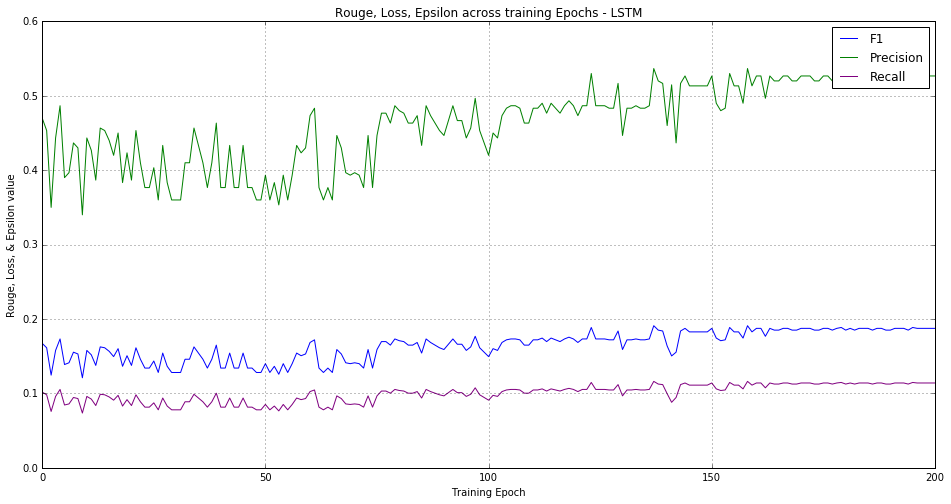
\includegraphics[width=\textwidth]{dqn_with_base}
    \caption{ \scriptsize (a): DQN with base exploration rate}
  \end{minipage}
  \hfill
  \begin{minipage}[b]{0.4\textwidth}
    \captionsetup{labelformat=empty}
    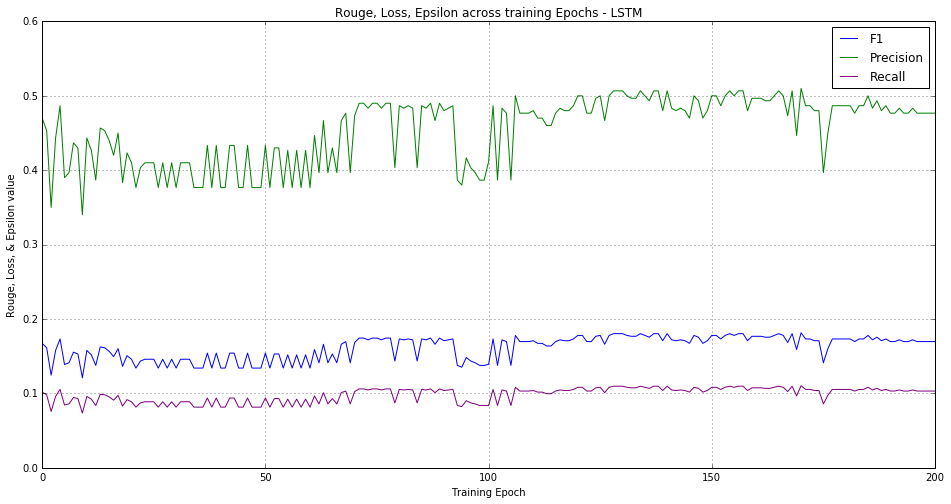
\includegraphics[width=\textwidth]{dqn_no_base}
    \caption{\scriptsize (b): DQN without base exploration rate}
  \end{minipage}
    \captionsetup{labelformat=empty}
    \caption{\textbf{Figure 2: DQN-LSTM Hyperparameter Experiments}}
\end{figure}

\subsection{Hyperparameters}
Different experiments were done to study the effect of each hyperparameter on the model.  Specifically, we evaluate (1) the settings of $K$ to assess the impact on the final predicted summary, (2) values of $\gamma$ to understand the effects on the parameter updates, (3) the memory size, $ | D |$ on the speed of convergence, and (4) the base exploration rate on the states explored. We present several figures visualizing the impact using different settings of the hyperparameters in our model in \textbf{Figure 3} on a smaller subset of the data; specifically, we use the first sentence from the first 100 articles for all but three of the queries, which are left as test data. 

\begin{figure}[h]
    \centering
    \fbox{
\includegraphics[scale=0.35]{perf}}
    \captionsetup{labelformat=empty}
    \caption{\textbf{Figure 3: DQN-LSTM Hyperparameter Experiments}}
\end{figure}

\section{Results}
We evaluate our learned extracted summaries on ROUGE-N F1, Recall, and Precision on the full set of nuggets averaged across all of the queries on the full predicted summary $\tilde{Y}_d$, $\forall d \in \mathcal{D}$. The hyperparameters for the three neural networks were set using cross-validation as described in the previous section. We present the performance of our DQN-LSTM against random action, bag-of-words and bag-of-bigrams multi-layered perceptrons in \textbf{Table 1}. 

\begin{center}
\begin{tabular}{  l | c | c | c  }
	\multicolumn{4}{c}{\textbf{Table 1}: Rouge Evaluation} \\
	\hline
	Model  & F1 & Recall & Precision  \\ \hline \hline
	Random  & \color{ red} - - & \color{ red} - -  & \color{ red} - -\\ 
	DQN-BOW  & \color{ red} - - & \color{ red} - -  & \color{ red} - -\\
	DQN-BiBOW  & \color{ red} - - & \color{ red} - -  & \color{ red} - -\\
	DQN-LSTM  & \color{ red}  - - & \color{ red} - -  & \color{ red} - -\\ \hline
	\hline
	\multicolumn{4}{l}{\footnotesize Average Rouge of the extracted summaries against} \\
	\multicolumn{4}{l}{\footnotesize the gold standard summaries for 3 of the 25 queries} \\
	\multicolumn{4}{l}{\footnotesize  on the first 10,000 articles of each query.} \\
	\hline
\end{tabular}
\end{center}

\section{Conclusion}
We have presented an end-to-end deep reinforcement learning architecture to learn an extraction policy for multi-document summarization. By treating the incoming sentence streams from different documents as inputs into a recurrent neural network and by backpropagating the action selected, we are able to learn both a richer embedding representation of the three input components and a robust extraction policy. 

Future research could consider modifying the extractive policy into one that generates a sequence. Sequence-to-sequence models \cite{sutskever2014sequence} have shown wide success in language translation and could be a useful model for the summarization of multiple documents.

\bibliography{DeepNLPQLearning}

\end{document}